\subsection{Intelligent experiments through real-time AI}
{{\footnotesize
\noindent Research and Development demonstrator for real-time processing of high-rate tracking data from the sPHENIX detector (RHIC) and future EIC systems. Uses GNNs with hls4ml for FPGA-based trigger generation to identify rare events (heavy flavor, DIS electrons) within 10 micros latency. Demonstrated improved accuracy and latency on Alveo/FELIX platforms.


\begin{description}[labelwidth=4cm, labelsep=1em, leftmargin=4cm, itemsep=0.1em, parsep=0em]
  \item[date:] 2025-01-08
  \item[version:] v1.0
  \item[last\_updated:] 2025-01
  \item[expired:] unknown
  \item[valid:] yes
  \item[valid\_date:] 2025-01-08
  \item[url:] \href{https://arxiv.org/pdf/2501.04845}{https://arxiv.org/pdf/2501.04845}
  \item[doi:] 10.48550/arXiv.2501.04845
  \item[domain:] Instrumentation and Detectors; Nuclear Physics; Particle Physics
  \item[focus:] Real-time FPGA-based triggering and detector control for sPHENIX and future EIC
  \item[keywords:]
    - FPGA
    - Graph Neural Network
    - hls4ml
    - real-time inference
    - detector control
  \item[licensing:] CC BY-NC-ND 4.0
  \item[task\_types:]
    - Trigger classification
    - Detector control
    - Real-time inference
  \item[ai\_capability\_measured:]
    - Low-latency GNN inference on FPGA
  \item[metrics:]
    - Accuracy (charm and beauty detection)
    - Latency (micros)
    - Resource utilization (LUT/FF/BRAM/DSP)
  \item[models:]
    - Bipartite Graph Network with Set Transformers (BGN-ST)
    - GarNet (edge-classifier)
  \item[ml\_motif:]
    - Real-time
  \item[type:] Model
  \item[ml\_task:]
    - Supervised Learning
  \item[solutions:] Solution details are described in the referenced paper or repository.
  \item[notes:] Achieved \textasciitilde{}97.4\% accuracy for beauty decay triggers; sub-10 micros latency on Alveo U280; hit-based FPGA design via hls4ml and FlowGNN.

  \item[contact.name:] Jakub Kvapil
  \item[contact.email:] Jakub.Kvapil@lanl.gov
  \item[datasets.links.name:] Internal simulated tracking data (sPHENIX and EIC DIS-electron tagger)
  \item[results.links.name:] ChatGPT LLM
  \item[fair.reproducible:] True
  \item[fair.benchmark\_ready:] False
  \item[id:] intelligent\_experiments\_through\_real-time\_ai
  \item[Citations:] \cite{kvapil2025intelligentexperimentsrealtimeai}
\end{description}

{\bf Ratings:} ~ \\

\begin{tabular}{p{0.15\textwidth} p{0.07\textwidth} p{0.7\textwidth}}
\hline
Rating & Value & Reason \\
\hline
dataset & 2 & Dataset is internal and not publicly available or FAIR-compliant
 \\
documentation & 3 & No public GitHub or complete pipeline documentation
 \\
metrics & 3 & Metrics relevant but not supported by evaluation scripts or baselines
 \\
reference\_solution & 3 & No public or reproducible implementation released
 \\
software & 3 & No containerized or open-source setup provided
 \\
specification & 4 & Architectural/system specifications are incomplete
 \\
\hline
\end{tabular}

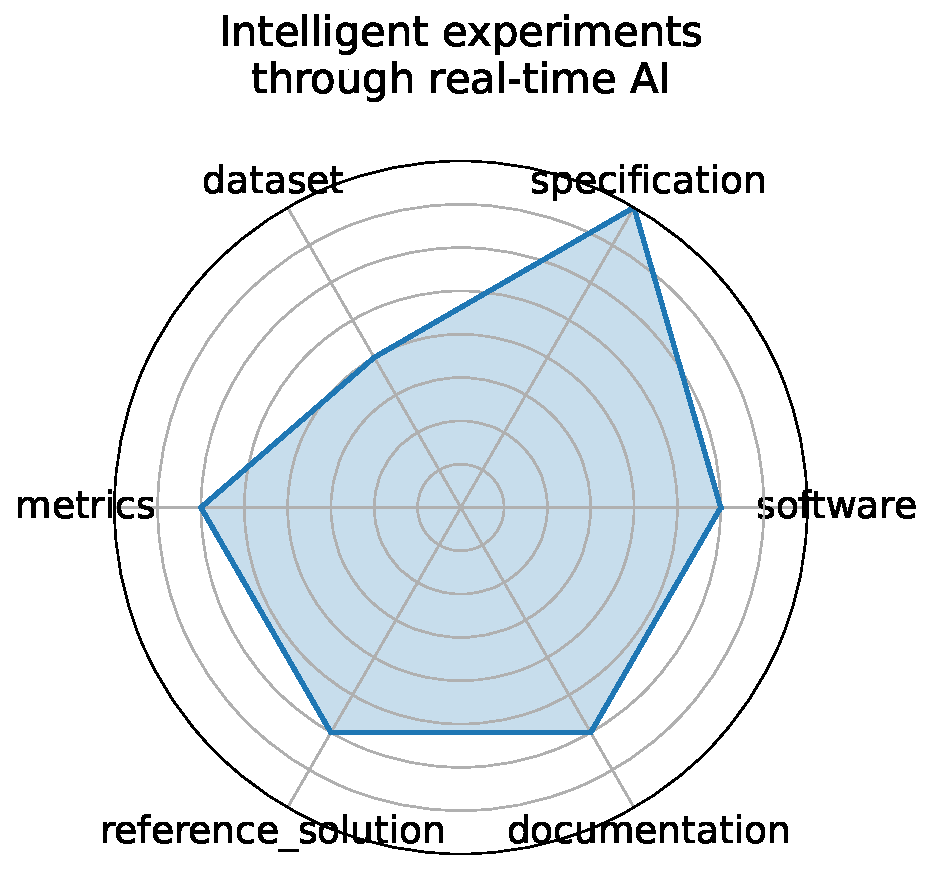
\includegraphics[width=0.2\textwidth]{intelligent_experiments_through_real-time_ai_radar.pdf}
}}
\clearpage